\documentclass[a4paper]{article}
\usepackage[english]{babel}
\usepackage[utf8]{inputenc}
\usepackage{amsmath}
\usepackage{graphicx}
\usepackage[colorinlistoftodos]{todonotes}
\graphicspath{{images/}}
\usepackage{wrapfig}
\usepackage{float}
\usepackage{parskip}
\usepackage{fancyhdr}
\usepackage{multicol}
\usepackage{vmargin}


\title{Actividad 2: Elementos de la programación Python 1}

\author{Paulina Valenzuela Coronado}

\date{\today}

\begin{document}
\maketitle

\section{Introducción}
En esta actividad se realizaron diferentes códigos en lenguaje phyton.
Phyton es Python es un lenguaje de programación interpretado cuya filosofía hace hincapié en una sintaxis que favorezca un código legible.

Se trata de un lenguaje de programación multiparadigma, ya que soporta orientación a objetos, programación imperativa y, en menor medida, programación funcional. Es un lenguaje interpretado, usa tipado dinámico y es multiplataforma.

Es administrado por la Python Software Foundation. Posee una licencia de código abierto, denominada Python Software Foundation License,1 que es compatible con la Licencia pública general de GNU a partir de la versión 2.1.1, e incompatible en ciertas versiones anteriores.


\section{Programas}
\begin{itemize}
\item \textbf{Programa 1} \\ 
Se deja caer una pelota desde el techo de una torre de altura h. Se desea saber el tiempo que tarda la pelota en llegar al suelo, ignorando la fricción del aire. Para esto se pide la altura de la torre y se regresa el tiempo.



\begin{figure}[H]
	\centering
	\includegraphics[height=2cm]{1.jpg}
\end{figure}

\item \textbf{Programa 2} \\
Un satélite orbita la Tierra a una altura h, con un periodo T en segundos. La altitud está dada por $$(R + h)^3 = (GMT^2)/(4 pi^2) $$, donde $G = 6.67 x 10^-11 \frac{m^3}{Kg m^2}$ es la constante de Gravitación Universal de Newton, $M = 5.97 x 10^24 kg$ es la masa de la Tierra y $R=6371$ km es su radio.
Este programa pide al usuario ingresar el valor deseado de T y regresa la altura h correspondiente en metros.



\begin{figure}[H]
	\centering
	\includegraphics[height=3cm]{2.jpg}
\end{figure}

\item \textbf{Programa 3} \\
Este programa calcula las coordenadas esféricas $(r, \theta, \phi)$ a partir de las coordenadas cartesianas $(x,y,z)$.

\begin{figure}[H]
	\centering
	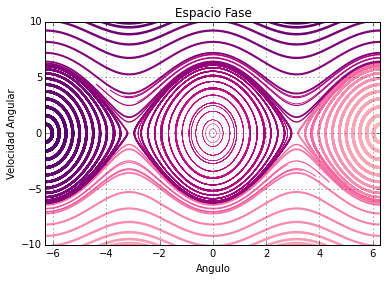
\includegraphics[height=4cm]{3.jpg}
\end{figure}

\item \textbf{Programa 4} \\
Sabemos que los números pares son divisibles entre 2, es decir que su residuo es cero (2n), mientras que los impares tienen residuo 1 (2n+1). El siguiente código admite 2 enteros, y utiliza el control while (mientras que).Al ingresar los dos números enteros, el programa espera a que $(m+n)/2==0$ para decirte si uno es impar. Si este no ocurre el programa solo te dirá que números utilizaste.


\begin{figure}[H]
	\centering
	\includegraphics[height=4cm]{4.jpg}
\end{figure}

\item \textbf{Programa 5} \\
Este programa imprime la secuencia de números de Catalan menores o iguales a 1000,000, que son dados por la fórmula de recurrencia:

$C0 = 1, C(n+1) = \frac{2(2n+1)}{(n+2)*Cn}$

\begin{figure}[H]
	\centering
	\includegraphics[height=7cm]{5.jpg}
\end{figure}

\end{itemize}

\end{document}